\section{Software Framework and Tools}\label{sec:framework}

%Experimental physics data analysis in a collaborative environment has historically involved a computing model based on self-contained, monolithic software applications running in batch-processing mode. This model, if not organized properly, can result in inefficiencies in terms of deployment, maintenance, response to program errors, update propagation, scalability and fault-tolerance. Over time, experimental configurations have become more diverse and compute capacity has expanded at a rate consistent with Moore's Law. As a consequence, compute applications have become much more complex, with significant interaction between diverse program components.  This can lead to computing systems so complex and intertwined that the programs become difficult to maintain and extend. Modifying a feature in one class often involves changes in several other classes, thereby increasing the needed development time and effort. What starts small and simple, inevitably grows into a complicated scheme of interconnected algorithms. At some point, to prevent further growth in complexity, the software has to be shielded from contributors, preventing essential software evolution and optimization. The only way to bypass this highly guarded system is software fragmentation, making the physics data processing validation process quite arduous.

%%%%%%%%%%%%%%%%%%%%%%%%%%%%%%%%%%%%%%%%%%%%%%%%%%%%%%%%%%
\begin{figure*}
\centering
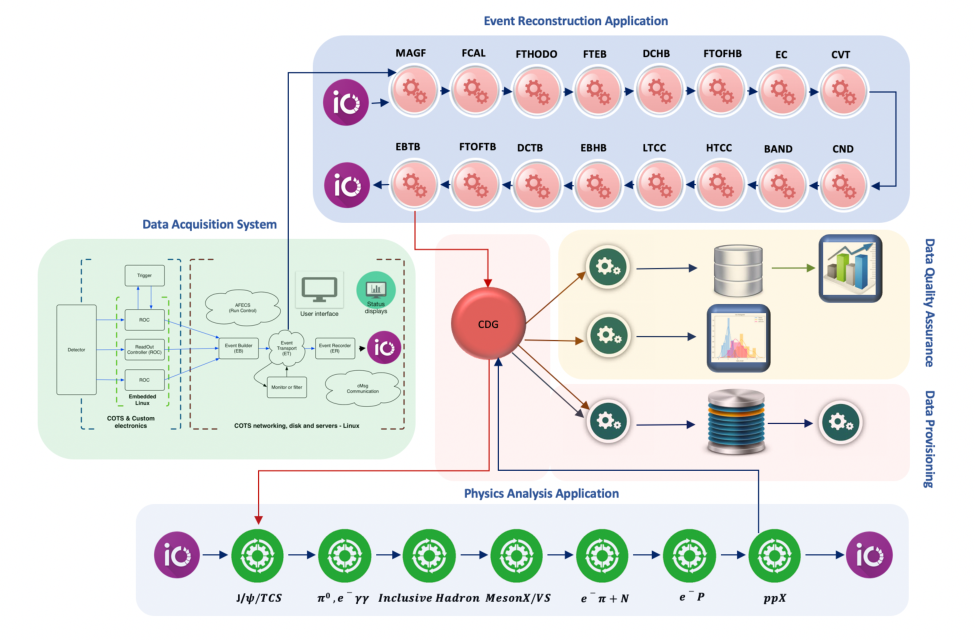
\includegraphics[width=0.8\textwidth]{pics/clara-overview.pdf}
\caption{Overview of the CLAS12 CLARA data processing framework.  Individual detector subsystem reconstruction applications can be linked to. form the full event reconstruction chain, including  data processing, data quality monitoring, and physics analysis applications.}
\label{fig:clara-overview}
\end{figure*}
%%%%%%%%%%%%%%%%%%%%%%%%%%%%%%%%%%%%%%%%%%%%%%%%%%%%%%%%%%%
Nuclear and particle physics data processing applications have a guarantee a long lifetime, equivalent or larger than the multi-year duration of the corresponding experiment. The ability to upgrade and adapt technologies is therefore essential. Hence, data processing applications should be organized in a way that easily permits the upgrade of aged software components and the inclusion of new ones, with  no need for major redesign or structural changes. In addition, support for software evolution and diversification (e.g. compatibility with heterogeneous hardware structures, such as FPGAs, GPGPUs, etc.) is important as it results in more efficient and robust data processing applications.


Following this principles, CLAS12 reconstruction and analysis relies on a reactive, data-stream processing framework called CLARA
\cite{clara-2011,clara-service,framework,clara-2016} that adopts a service-oriented architecture to build the relevant
software applications. 

Software applications designed within the CLAS12 CLARA data processing framework are composed of interlocking building blocks
(bricks), called micro-services. Micro-services are linked together by data-stream pipes.  The technology
(e.g. high-level programming language, hardware deployment details) as well as the algorithmic solutions used to process
data (see Fig.~\ref{fig:clara-overview}) are encapsulated. A micro-service has inputs, processes data and produces output data. Inputs and outputs data and organized in ``banks'' whose structure is configured by the specific service developer.
A micro-service reacts on a streaming data quantum in its input, processes it, and passes processed data quanta to the next micro-service in the data-flow path. 

The CLAS12 data processing applications execute according to the rules of data-flow instead of a more traditional
programming approach, where sequential series of instructions (lines of code) are written to perform a required algorithm. The flow of data between micro-services in the application determines
the execution order of micro-services within the application. These features make the data paths between application building blocks to be the application designer’s main focus. As a result, the CLAS12 data processing application is versatile and flexible, since
the application building blocks can be improved individually and replaced with no need of structure changes in the framework. 
The CLARA data-stream pipe is a data bus based on the xMsg messaging system that supports various protocols such as MPI, pub-sub, p2p, inproc, and shared memory. The CLARA orchestrator, i.e. the process level workflow management systems, controls the overall process execution. 

In the case of the CLAS12 event reconstruction application, the micro-services are built as extension of a template reconstruction engine which includes common components such as engine initialization and events processing methods. This approach strongly reduces and simplifies the development of an individual micro-service by enforcing a common structure. 

SHOULD ADD SOMETHING ON EVENT PARALLELIZATION AND MULTI-HW SUPPORT.

\subsection{Common Tools}
\label{common-tools}

The offline software of the CLAS12 project aims at providing tools to
the experimental collaboration that allow design, simulation, and data analysis to proceed
in an efficient, repeatable, and understandable way. As much as
possible, software-engineering-related details should be hidden from
users, allowing them to concentrate on the algorithms and physics.
To facilitate code development for the detector subsystems of CLAS12, and for detector-specific reconstruction output
analysis used for particle identification and overall event reconstruction,
the software was designed to provide libraries that are commonly used by all the reconstruction
packages.  These libraries, referred to as ``common tools'' provide means to avoid code replication and aid in software maintainability.

The common tools consist of various packages, each having a specific purpose and functionality. Below we discuss
the main packages used in the reconstruction software.

\subsubsection{Geometry}

Due to the complexity of the geometry of CLAS12 detector subsystems, an interface was developed
to provide classes and software tools that are used to describe the geometry of all subsystem in an unified way.

A library of primitives was developed to provide geometrical objects needed to represent by all geometry detector subsystem
and for geometrical object transformations.  These primitives include lines, planes and various shapes (e.g.
cubes, trapezoids, etc.).  They provide the functionality needed
to represent the detector subsystem components in the reconstruction frames, to take into account geometrical distortions
and to translate and rotate detector components, which is particularly relevant for alignment purposes.
Furthermore, geometry tools provide methods to track particles through volumes, and return information used to determine
track trajectories, such as line to surface intersections, ray tracing through objects, distance of closest approach to a line or surface.

The CLAS12 geometry library is initialized from database, where the detector geometry key parameters are stored for maximum flexibility, and ensures consistency between the geometry implementation used in CLAS12 simulation, reconstruction and event visualization packages. The library in fact provides the input geometries for the GEANT4 simulations package (GEMC)~\cite{sim-nim}, the reconstruction application and the CLAS12 Event Display (CED).

To facilitate the detector geometries implementation, visualization capalities were included in the geometry library. Fig.~\ref{fig:detectorview} shows a view of part of the CLAS12 spectrometer using this functionality.

\begin{figure}
\centering
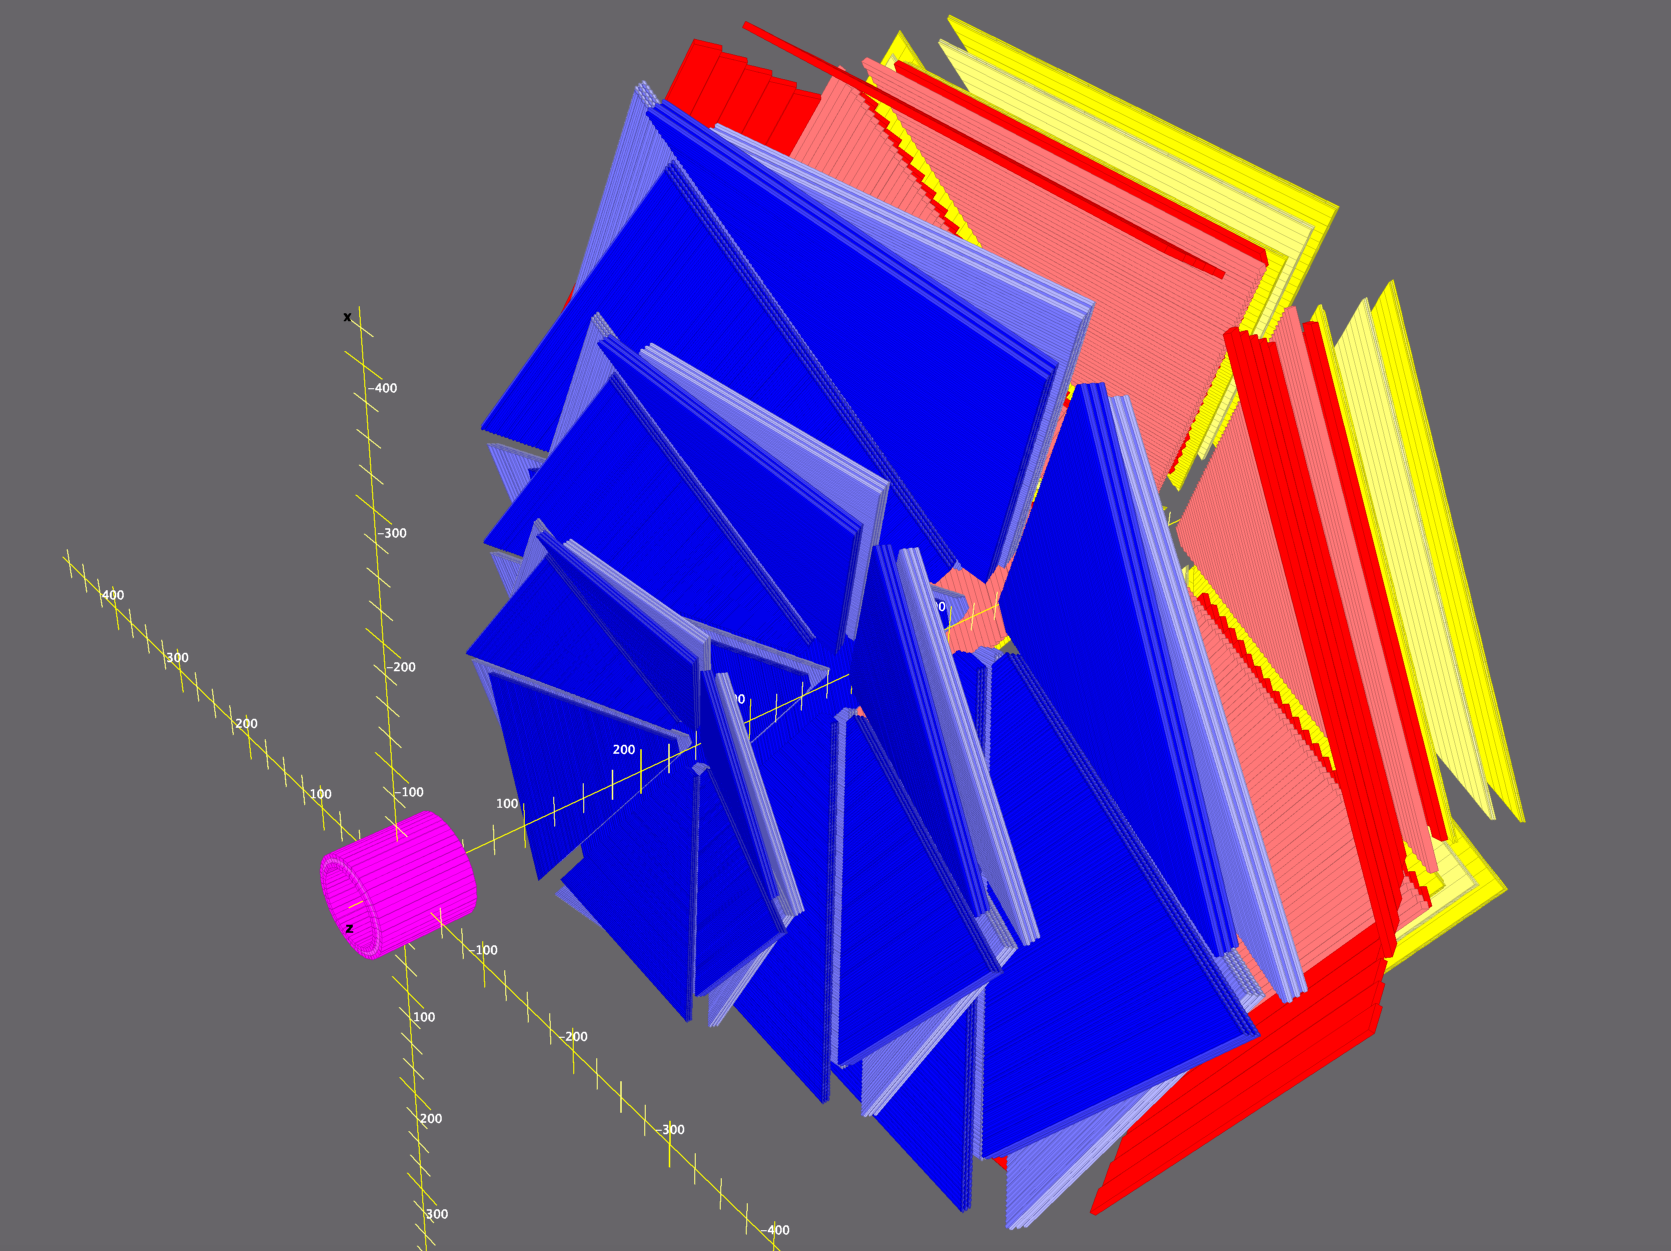
\includegraphics[width=1.0\columnwidth]{reconstruction/pics/detectorview.png}
\caption{Visualization of part of the CLAS12 spectrometer via the geometry package. From left to right, the Central Neutron Detector (CND) in magenta, the Drift Chambers (DC) in blue, the Forward Time of Flight (FTOF) in red, the Electromagnetic Calorimeter (ECAL) in yellow are shown.}
\label{fig:detectorview}
\end{figure}
\subsubsection{Databases}

The Calibration Constant Data Base (CCDB) software package was developed at Jefferson Lab for the GlueX experiment
in HallD~\cite{gluex}.  CCDB provides the functionality for storing and accessing structured tables in MySQL-based and SQLite portable databases.
The CLAS12 reconstruction packages use the CCDB application programming interface to create and access
tables that contain detector geometry and calibration constants, as well as maps used for decoding raw data.

The CCDB package creates
tables that link constants to specific runs (using timestamps) and store different variations of constants depending on run
conditions. CLAS12 software tools employ an Application Programming Interface (API) that parses database tables and creates
structured maps of constants stored in  memory by detector sector, layer and component. This allows fast retrieving of the
constants.

The CLAS12 database access tools have been developed to avoid bottlenecks that might result from multiple multi-threaded
services accessing the database to retrieve constants.  An interface has been designed to fetch the constants
on demand and cache them for further requests. In this approach each service will request the
constants it requires on one thread and each subsequent request by a new thread will be provided by the cached values.

\subsubsection{Plotting and Analysis Tools}

For ease of integration with the reconstruction software tools and packages, the plotting tools used for data
calibration, monitoring and analysis was developed in the JAVA programming language.

The plotting software, called {\it groot}, developed at Jefferson Lab for CLAS12 is tailored to have a programming
interface similar to the CERN data analysis package, ROOT, and provides the the necessary functionalities for histogram and graphs creation, filling and manipulation as well as for fitting using the JAVA-based MINUIT library available from the JHEP repositories. This has been the base for the development of detector monitoring and calibration suites (see Sec.~\ref{sec:calibration}.

These same tools can be used for analysis purposes. In addition, the analysis package contains classes for four-vector manipulations and physics quantities extractions and
analysis methods (e.g. $Q^2, W$, boosts, etc.).

\subsubsection{Magnetic Field Package}
The magnetic field package {\it magfield} used by CLAS12 reconstruction creates
binary field maps from engineering models of the CLAS12 torus and solenoid. It employs
a common self-described binary format, with a header containing meta-data describing
the pedigree of the field, its grid coordinate system, and the coordinate system
used by the field values. For example, the CLAS12 torus has a cylindrical grid
but Cartesian field components. The same magfield package provides the trilinear
interpolation of the field. Given that the field is often requested at a sequence
of points all contained within a single grid cell, magfield uses time-saving
software “probes” to cache nearest neighbors.

\subsubsection{Swimmer Package}
The swimmer package, in conjunction with the magfield package, is used by the CLAS12
reconstruction to integrate charged particles through the CLAS12 solenoid and torus.
It uses a fourth order (with 5th order corrections) adaptive step-size Runge-Kutta integrator
with single-step advancement achieved through a configurable Butcher tableau advancer.
There are a number of convenience methods for swimming to a plane, to the closest
point on a line, and to a specified value of a given coordinate such as z. For
forward swimming in CLAS12, the swimmer can reduce the dimensionality of the state
vector (and consequently run faster) by changing the independent variable from
the pathlength to the z coordinate.

